% -*- Mode:TeX -*-

%% IMPORTANT: The official thesis specifications are available at:
%%            http://libraries.mit.edu/archives/thesis-specs/
%%
%%            Please verify your thesis' formatting and copyright
%%            assignment before submission.  If you notice any
%%            discrepancies between these templates and the 
%%            MIT Libraries' specs, please let us know
%%            by e-mailing thesis@mit.edu

%% The documentclass options along with the pagestyle can be used to generate
%% a technical report, a draft copy, or a regular thesis.  You may need to
%% re-specify the pagestyle after you \include  cover.tex.  For more
%% information, see the first few lines of mitthesis.cls. 

%\documentclass[12pt,vi,twoside]{mitthesis}
%%
%%  If you want your thesis copyright to you instead of MIT, use the
%%  ``vi'' option, as above.
%%
%\documentclass[12pt,twoside,leftblank]{mitthesis}
%%
%% If you want blank pages before new chapters to be labelled ``This
%% Page Intentionally Left Blank'', use the ``leftblank'' option, as
%% above. 

\documentclass[12pt,vi,oneside]{mitthesis}
\usepackage{lgrind}
%% These have been added at the request of the MIT Libraries, because
%% some PDF conversions mess up the ligatures.  -LB, 1/22/2014
\usepackage{cmap}
\usepackage[T1]{fontenc}
\pagestyle{plain}

%% This bit allows you to either specify only the files which you wish to
%% process, or `all' to process all files which you \include.
%% Krishna Sethuraman (1990).

%\typein [\files]{Enter file names to process, (chap1,chap2 ...), or `all' to
%process all files:}
%\def\all{all}
%\ifx\files\all \typeout{Including all files.} \else \typeout{Including only \files.} \includeonly{\files} \fi

% Overwrite some commands
\renewcommand{\contentsname}{Inhaltsverzeichnis}

\begin{document}

% -*-latex-*-
% 
% For questions, comments, concerns or complaints:
% thesis@mit.edu
% 
%
% $Log: cover.tex,v $
% Revision 1.8  2008/05/13 15:02:15  jdreed
% Degree month is June, not May.  Added note about prevdegrees.
% Arthur Smith's title updated
%
% Revision 1.7  2001/02/08 18:53:16  boojum
% changed some \newpages to \cleardoublepages
%
% Revision 1.6  1999/10/21 14:49:31  boojum
% changed comment referring to documentstyle
%
% Revision 1.5  1999/10/21 14:39:04  boojum
% *** empty log message ***
%
% Revision 1.4  1997/04/18  17:54:10  othomas
% added page numbers on abstract and cover, and made 1 abstract
% page the default rather than 2.  (anne hunter tells me this
% is the new institute standard.)
%
% Revision 1.4  1997/04/18  17:54:10  othomas
% added page numbers on abstract and cover, and made 1 abstract
% page the default rather than 2.  (anne hunter tells me this
% is the new institute standard.)
%
% Revision 1.3  93/05/17  17:06:29  starflt
% Added acknowledgements section (suggested by tompalka)
% 
% Revision 1.2  92/04/22  13:13:13  epeisach
% Fixes for 1991 course 6 requirements
% Phrase "and to grant others the right to do so" has been added to 
% permission clause
% Second copy of abstract is not counted as separate pages so numbering works
% out
% 
% Revision 1.1  92/04/22  13:08:20  epeisach

% NOTE:
% These templates make an effort to conform to the MIT Thesis specifications,
% however the specifications can change.  We recommend that you verify the
% layout of your title page with your thesis advisor and/or the MIT 
% Libraries before printing your final copy.
\title{Nature-Inspired Algorithms}

\author{Yves Beutler}
% If you wish to list your previous degrees on the cover page, use the 
% previous degrees command:
%       \prevdegrees{A.A., Harvard University (1985)}
% You can use the \\ command to list multiple previous degrees
%       \prevdegrees{B.S., University of California (1978) \\
%                    S.M., Massachusetts Institute of Technology (1981)}
\department{BFH Technik und Informatik}

% If the thesis is for two degrees simultaneously, list them both
% separated by \and like this:
% \degree{Doctor of Philosophy \and Master of Science}
\degree{Bachelor of Science BFH in Informatik}

% As of the 2007-08 academic year, valid degree months are September, 
% February, or June.  The default is June.
\degreemonth{Juni}
\degreeyear{2019}
\thesisdate{10. Juni, 2019}

%% By default, the thesis will be copyrighted to MIT.  If you need to copyright
%% the thesis to yourself, just specify the `vi' documentclass option.  If for
%% some reason you want to exactly specify the copyright notice text, you can
%% use the \copyrightnoticetext command.  
%\copyrightnoticetext{\copyright IBM, 1990.  Do not open till Xmas.}

% If there is more than one supervisor, use the \supervisor command
% once for each.
\supervisor{Dr. Mascha Kurpicz-Briki}{Betreuende Professorin}

% This is the department committee chairman, not the thesis committee
% chairman.  You should replace this with your Department's Committee
% Chairman.
%\chairman{Arthur C. Smith}{Chairman, Department Committee on Graduate Theses}
%\chairman{ d}{a }

% Make the titlepage based on the above information.  If you need
% something special and can't use the standard form, you can specify
% the exact text of the titlepage yourself.  Put it in a titlepage
% environment and leave blank lines where you want vertical space.
% The spaces will be adjusted to fill the entire page.  The dotted
% lines for the signatures are made with the \signature command.

\maketitle

% The abstractpage environment sets up everything on the page except
% the text itself.  The title and other header material are put at the
% top of the page, and the supervisors are listed at the bottom.  A
% new page is begun both before and after.  Of course, an abstract may
% be more than one page itself.  If you need more control over the
% format of the page, you can use the abstract environment, which puts
% the word "Abstract" at the beginning and single spaces its text.

%% You can either \input (*not* \include) your abstract file, or you can put
%% the text of the abstract directly between the \begin{abstractpage} and
%% \end{abstractpage} commands.

% First copy: start a new page, and save the page number.
\cleardoublepage
% Uncomment the next line if you do NOT want a page number on your
% abstract and acknowledgments pages.
% \pagestyle{empty}
\setcounter{savepage}{\thepage}
\begin{abstractpage}
% $Log: abstract.tex,v $
% Revision 1.1  93/05/14  14:56:25  starflt
% Initial revision
% 
% Revision 1.1  90/05/04  10:41:01  lwvanels
% Initial revision
% 
%
%% The text of your abstract and nothing else (other than comments) goes here.
%% It will be single-spaced and the rest of the text that is supposed to go on
%% the abstract page will be generated by the abstractpage environment.  This
%% file should be \input (not \include 'd) from cover.tex.
DRAFT:

Nature-Inspired Algorithms können dort eingesetzt werden, wo traditionelle
Problemlösungsmethoden nicht funktionieren. Einige dieser Algorithmen haben
sich als äusserst performant und robust erwiesen und werden heute zur Problemlösung
in den unterschiedlichsten Anwedungsgebieten eingesetzt. Zu der Gruppe der Nature-Inspired
Algorithms gehören beispielsweise Evolutionäre-Algorithmen, welche starke Ähnlichkeiten zu
Darwins Evolutionstheorie mit seinem bekannten Zitat von 'Survival of the fittest aufweisen'.
Weiter werden Schwarm- und Neuronale-Algorithmen thematisiert, wobei aktuell die letzteren,
durch die neusten Grafikkartengenerationen herbeigeführt, einen erneuten Aufschwung erleben
dürfen. Nach einer kurzen Übersicht der einzelnen Gruppen wird jede behandelte Unterart der
Nature-Inspired Algorithms durch einen ausgewählten Algorithmus im Detail veranschaulicht.

Ziel dieser Arbeit ist es, eine Einführung in die Thematik von Nature-Inspired Algorithms und ihren
Einsatzmöglichkeiten zu geben und die bekanntesten Unterarten mit ausgesuchten Algorithmen im Detail
zu erläutern.


\end{abstractpage}

% Additional copy: start a new page, and reset the page number.  This way,
% the second copy of the abstract is not counted as separate pages.
% Uncomment the next 6 lines if you need two copies of the abstract
% page.
% \setcounter{page}{\thesavepage}
% \begin{abstractpage}
% % $Log: abstract.tex,v $
% Revision 1.1  93/05/14  14:56:25  starflt
% Initial revision
% 
% Revision 1.1  90/05/04  10:41:01  lwvanels
% Initial revision
% 
%
%% The text of your abstract and nothing else (other than comments) goes here.
%% It will be single-spaced and the rest of the text that is supposed to go on
%% the abstract page will be generated by the abstractpage environment.  This
%% file should be \input (not \include 'd) from cover.tex.
DRAFT:

Nature-Inspired Algorithms können dort eingesetzt werden, wo traditionelle
Problemlösungsmethoden nicht funktionieren. Einige dieser Algorithmen haben
sich als äusserst performant und robust erwiesen und werden heute zur Problemlösung
in den unterschiedlichsten Anwedungsgebieten eingesetzt. Zu der Gruppe der Nature-Inspired
Algorithms gehören beispielsweise Evolutionäre-Algorithmen, welche starke Ähnlichkeiten zu
Darwins Evolutionstheorie mit seinem bekannten Zitat von 'Survival of the fittest aufweisen'.
Weiter werden Schwarm- und Neuronale-Algorithmen thematisiert, wobei aktuell die letzteren,
durch die neusten Grafikkartengenerationen herbeigeführt, einen erneuten Aufschwung erleben
dürfen. Nach einer kurzen Übersicht der einzelnen Gruppen wird jede behandelte Unterart der
Nature-Inspired Algorithms durch einen ausgewählten Algorithmus im Detail veranschaulicht.

Ziel dieser Arbeit ist es, eine Einführung in die Thematik von Nature-Inspired Algorithms und ihren
Einsatzmöglichkeiten zu geben und die bekanntesten Unterarten mit ausgesuchten Algorithmen im Detail
zu erläutern.


% \end{abstractpage}

\cleardoublepage

\section*{Danksagung}

Tbd..

% Special thanks to Dr. Mascha Kurpicz-Briki for supporting me during the semester
% while I was working on this term paper and Natalie Kuster for providing me
% with additional information about genetic algorithms and especially data science
% related topics I covered in the next few pages. \\ \\
% Another thank you to Kieran Willis for proofreading my term paper.

%%%%%%%%%%%%%%%%%%%%%%%%%%%%%%%%%%%%%%%%%%%%%%%%%%%%%%%%%%%%%%%%%%%%%%
% -*-latex-*-

% Some departments (e.g. 5) require an additional signature page.  See
% signature.tex for more information and uncomment the following line if
% applicable.
% % -*- Mode:TeX -*-
%
% Some departments (e.g. Chemistry) require an additional cover page
% with signatures of the thesis committee.  Please check with your
% thesis advisor or other appropriate person to determine if such a 
% page is required for your thesis.  
%
% If you choose not to use the "titlepage" environment, a \newpage
% commands, and several \vspace{\fill} commands may be necessary to
% achieve the required spacing.  The \signature command is defined in
% the "mitthesis" class
%
% The following sample appears courtesy of Ben Kaduk <kaduk@mit.edu> and
% was used in his June 2012 doctoral thesis in Chemistry. 

\begin{titlepage}
\begin{large}
This doctoral thesis has been examined by a Committee of the Department
of Chemistry as follows:

\signature{Professor Jianshu Cao}{Chairman, Thesis Committee \\
   Professor of Chemistry}

\signature{Professor Troy Van Voorhis}{Thesis Supervisor \\
   Associate Professor of Chemistry}

\signature{Professor Robert W. Field}{Member, Thesis Committee \\
   Haslam and Dewey Professor of Chemistry}
\end{large}
\end{titlepage}


\pagestyle{plain}
  % -*- Mode:TeX -*-
%% This file simply contains the commands that actually generate the table of
%% contents and lists of figures and tables.  You can omit any or all of
%% these files by simply taking out the appropriate command.  For more
%% information on these files, see appendix C.3.3 of the LaTeX manual. 
\tableofcontents
\newpage
\listoffigures
%% \newpage
%% \listoftables


%% This is an example first chapter.  You should put chapter/appendix that you
%% write into a separate file, and add a line \include{yourfilename} to
%% main.tex, where `yourfilename.tex' is the name of the chapter/appendix file.
%% You can process specific files by typing their names in at the 
%% \files=
%% prompt when you run the file main.tex through LaTeX.
\chapter{Einführung}

Seit dem Anbeginn unseres Planeten sah sich die Natur mit mehr oder weniger
komplexen Problemstellungen konfrontiert, um das Überleben ihrer Bewohner
sicherzustellen. Der Schlüssel zum Erfolg ist es, sich am besten auf die
naturgegebenen Umstände anzupassen. Ohne den Einklang mit der Natur wären die
Überlebenschancen einer jeden Spezies schwindend gering wenn nicht gar inexistent.
Seit Jahrzehnten adaptieren Menschen die Techniken aus der Natur und ihren Geschöpfen
um moderne Technologien auf ein neues Level zu befördern. Flugzeuge werden nach den
Flügelcharakteristiken von Zugvögeln konstruiert und neue Klebstoffe werden durch das
Studium von Geckofüssen mit ihren unglaublichen Hafteigenschaften entworfen. \cite{Cro14}

Wir dürfen nicht ausser Acht lassen, dass die Natur Millionen von Jahre in die Forschung
nach dem Schlüssel zum Überleben investierte und in den meisten Fällen scheiterte. Doch
die Natur gab nicht einfach auf, sondern justierte bestimmte Parameter um über die Zeit
zunehmend besser zu werden. Durch sich ständig ändernde Umstände sucht sie auch heute noch
nach Lösungen für zukünftige Spezien.

Wieso sollte die Menschheit nicht selbst von diesen Millionen von Jahren an Forschung profitieren?

\section{Anwendungsgebiete}

Nature-Inspired Algorithms werden meist dort eingesetzt, wo traditionelle Algorithmen keine oder
keine brauchbaren Ergebnisse liefern können. Häufig scheitern altbekannte Lösungsmodelle wenn mit
riesigen Datenmengen gearbeitet wird. Folgende Gegebenheiten können weitere Gründe sein, um auf
Nature-Inspired Algorithms zurückzugreifen:

\begin{enumerate}
    \item Die Anzahl möglicher Lösungen im Suchraum ist so immens gross, dass die Suche nach der bestmöglichen
          Lösung viel zu aufwändig wäre.
    \item Die Komplexität der Problemstellung ist derart hoch, dass nur vereinfachte Modelle bei der Problemlösung
          zum Einsatz kommen und dadurch keine aussagekräftigen Lösungen entstehen.
    \item Die Evaluierungsfunktion zur Bewertung einer möglichen Lösung variert mit der Zeit, so dass nicht nur eine
          sondern eine Vielzahl von Lösungen erforderlich ist.
\end{enumerate}

\cite[Kap. 1.2]{Bro11} \\

Eine weitverbreitete Eigenschaft von Nature-Inspired Algorithms ist die Kombination aus Regeln und Zufälligkeiten, um
natürliche Phänomene zu imitieren \cite{NH15}. Die Einsatzmöglichkeiten scheinen unendlich zu sein: 


\subsection{Optimierungen}
Häufige Anwendungsfälle dieser Algorithmen sind Optimierungen von Funktionen. Bei Optimierungen
handelt es sich in der Regel um die Suche nach einer Parameterkombination für eine gegebene Funktion $f$ um eine
Kostenfunktion zu minimieren oder eine Wertefunktion zu maximieren.

\subsection{Approximationen}
Die Approximation beschreibt meist eine Funktion $f$, welche möglichst nahe an eine Zielfunktion angenähert werden
möchte. Die approximierte Funktion $f$ wird aus einem Set an Beobachtungen\footnote{oftmals auch als $training$ $set$ aus
der Data Science bekannt} generiert. Solche Approximationen werden häufig für Image Recognition verwendet
und spielen ebenfalls eine wichtige Rolle bei der Klassifikation und dem Clustering von grossen Datenmengen.
%% This is an example first chapter.  You should put chapter/appendix that you
%% write into a separate file, and add a line \include{yourfilename} to
%% main.tex, where `yourfilename.tex' is the name of the chapter/appendix file.
%% You can process specific files by typing their names in at the 
%% \files=
%% prompt when you run the file main.tex through LaTeX.
\chapter{Evolutionäre Algorithmen}

Diese Subkategorie von Algorithmen wurde durch den natürlichen Prozess der Evolution
inspiriert. Charles Darwin begründete 1838 den Evolutionsprozess und das daraus resultierende
Überleben der jeweils am besten angepassten Individuen mit der natürlichen Selektion \cite{Wiki02}.
Diese stellt sicher, dass sich gut an den Lebensraum angepasst Lebewesen in der Natur
durchsetzen können, währenddessen weniger gut angepasste Individuen aussterben. Zudem
arbeitet die Natur nach dem 'Trial and Error' Prinzip. Dadurch werden Mutationen an
Lebewesen ausprobiert und bei positivem Effekt auf das Überleben der Spezies beibehalten,
bei einer Verminderung der Überlebenschancen jedoch wieder rückgängig gemacht. Dieser Prozess
ist sehr zeitaufwändig, jedoch nachhaltig wirksam. Viele Algorithmen wie beispielsweise
der Hill Climbing Algorithmus \cite{Anr18} wenden ebenfalls dieses Prinzip an.

\section{Genetische Algorithmen}

Die Genetischen Algorithmen sind die bekanntesten Vertreter aus der Gruppe der Evolutionären
Algorithmen. Sie orientierten sich an der Populationsgenetik und insbesondere an den Mendelschen
Regeln \cite{Mcc00}.
Bei Genetischen Algorithmen werden häufig Begriffe aus der Biologie verwendet. Die Anzahl an
möglichen Lösungen nennt man Population. Eine einzelne Lösungsvariante wird als Chromosom
bezeichnet, wohingegen diese wiederum aus einer Kombination an Variablen, in der Biologie Gene
genannt, bestehen. Wie aus der Grafik \ref{fig:genetics} zu entnehmen ist, besteht ein Chromosom
$A_n$ aus mehreren Genen.
\\
\begin{figure}[h!]
  \centering
  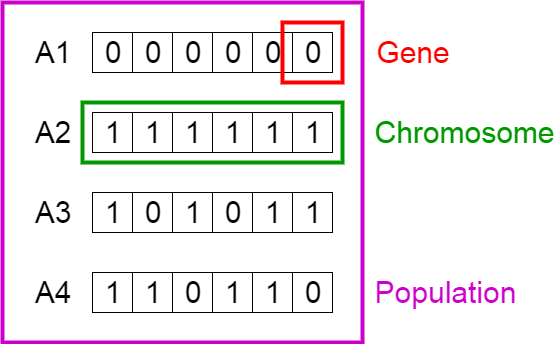
\includegraphics[scale=0.5]{resources/genetic_algorithms.png}
  \caption{Population, Chromosome und Gene \cite{Mal17}}
  \label{fig:genetics}
\end{figure}

Im folgenden werden die einzelnen Schritte erläutert, welche die Natur wie auch die Genetischen
Algorithmen durchlaufen, um eine Anfangspopulation schrittweise weiterzuentwickeln. Die Natur
sucht nach der erfolgsversprechendsten Lösung zum Überleben, wohingegen die Algorithmen
optimale Lösungen für ganz unterschiedliche Problemstellungen suchen. \cite{Mal17}

\subsection{Initiale Population}
Eine Population besteht aus mehreren unabhängigen Lösungen, im biologischen Kontext Chromosomen,
um eine bestimmte Problemstellung zu lösen. Bei den meisten Implementationen von Genetischen
Algorithmen wird ein Gen durch einen String repräsentiert. Bei Chromosomen eignen sich auch
Binärwerte um das Vorhandensein eines Gens auszuzeichnen.

\subsection{Selektion}
Anhand einer sogenannten Fitnessfunktion wird für jedes Individuum eine Punktzahl berechnet.
Die Punktzahl gibt darüber Auskunft, wie kompetitiv sich ein Individuum gegenüber einem anderen
verhält. Je höher dieser Wert, desto höher sind die Chancen, das besagtes Individuum von der
Selektion für die Reproduktion verwendet wird. Durch die Selektion können nur die fittesten
Individuen ihre Gene an die nächste Generation weitergeben und den schwächeren Individuen wird
der Reproduktionszyklus verwehrt.

\subsection{Kreuzung}
Der womöglich zentralste Bestandteil eines Genetischen Algorithmus ist die Kreuzung. Hier werden
aus den zuvor selektierten Individuen, einer Ansammlung der vielversprechendsten Lösungen, zwei
Individuen zur Paarung ausgewählt. Die beiden Ausgewählten tauschen ihre Gene bis zu einem bestimmten
Punkt, dem sogenannten Crossover Point, aus. Die restlichen Gene hinter diesem Punkt werden nicht
verändert. Durch diesen Prozess entstehen gleich zwei neue Individuen.

\subsection{Mutation}
Die Natur nutzt Mutationen aus, um die Artenvielfalt innerhalb einer Population zu gewährleisten.
Trotz der geringen Wahrscheinlichkeit kommt es vor, dass einzelne Gene, welche durch die Kreuzung
eigentlich vorhanden wären, nicht mehr vorhanden sind und umgekehrt. Ein Genetischer Algorithmus
flippt beispielsweise einzelne Variablen seiner Nachkommen. Durch die Mutation wird verhindert,
dass unser Algorithmus in einem lokalen Minimum stecken bleibt.

\subsection{Terminierung}
Ein Genetischer Algorithmus terminiert, sobald sich die nächste Generation nicht mehr merklich von
ihren Vorgängern unterscheidet. Man spricht oftmals auch von Konvergenz. Es ist jedem Algorithmus
selbst überlassen, wie lange ein Individuum in der Population überlebt. Häufig werden bei jedem
Reproduktionszyklus ein oder mehrere Individuen mit den niedrigsten Fitnesswerten aus der Population
gestrichen. In der Natur übernimmt der Tod diese Funktion.

\subsection{Beispiel Implementation}
Die einzelnen Schritte eines Genetischen Algorithmus sind in Listing A.1 durch
ein Python-Beispiel verdeutlicht. Die verwendete Fitnessfunktion ist sehr rudimentär
gehalten und berechnet lediglich die Summe der vorhandenen Gene. Die Population ist konvergiert,
wenn ein Individuum den Fitnesswert 5 erreicht, sprich alle Gene vorhanden sind.

Zweck dieses Listings ist es, den Ablauf eines Genetischen Algorithmus verständlich darzustellen.
Für eine bessere Übersicht wurden dazu uninteressante Teile des Codes gänzlich weggelassen.

\subsection{Vorteile}
Genetische Algorithmen haben gewisse Vorzüge bei der Lösung von komplexen
Problemstellungen gegenüber traditionellen Verfahren. Durch den modularen Aufbau
mit den drei Hauptfunktionen Selektion, Kreuzung und Mutation, lassen sich diese
Algorithmen einfach parallelisieren, was sich in einer besseren Rechenzeit bemerkbar
macht. Weiter generieren sie nicht nur eine Lösung sondern eine Vielzahl an möglichen
Lösungen, welche mit der Zeit immer bessere Ergebnisse liefern. \cite{Gou19}

\subsection{Anwendungsfälle}
Es existieren schier endlose Einsatzmöglichkeiten für Genetische Algorithmen. Sie werden unter anderem
zum Trainieren von Neuronalen Netzwerken eingesetzt, zur Berechnung von Fahrplänen wie auch den zu fahrenden
Routen (analog dem Traveling Salesman Problem), zur Konstruktion von Aerodynamischen Fahrzeugchassis in
der Luftfahrts- sowie in der Automobilbranche und häufig auch in der Finanzwirtschaft wie beispielsweise
zur dynamischen Preisberechnung \cite{Tut}.

\section{Genetic Programming}
Eine weitere Unterart der Evolutionären Algorithmen ist Genetic Programming. Ähnlich wie
bei den Genetischen Algorithmen ist Genetic Programming auch von den Mendelschen Regeln
inspiriert worden. Die Population besteht jedoch nicht wie bisher gezeigt aus einzelnen
Lösungen, sondern aus Programmen, welche eine Aufgabenstellung in unterschiedlicher
Qualität lösen können. Ziel ist es, dass diese Programme durch den Vererbungsprozess
von Generation zu Generation besser auf die jeweilige Problemstellung angepasst werden.
\cite{GenGP}

\subsection{Darstellungsformen}
Es stellt sich die Frage, wie eine Applikation repräsentiert werden kann, um anschliessend von
Genetic Programming optimiert werden zu können. Es existieren nebst Tree- und Stack-basierten
eine Lineare sowie eine Kartesische Darstellungsform. Im folgenden wird die Tree-basierte Form
genauer erläutert.

\begin{figure}[h!]
  \centering
  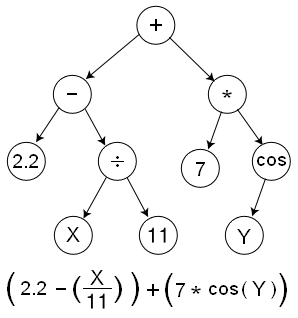
\includegraphics[scale=0.5]{resources/genetic_program_tree.png}
  \caption{Einfaches mathematisches Programm als Tree dargestellt \cite{Wiki01}}
  \label{fig:gp_tree}
\end{figure}

Wie in Grafik \ref{fig:gp_tree} erkennbar ist, werden die einzelnen Operationen in der Tree-basierten
Darstellungsweise durch Knoten repräsentiert. Die Operanden sind dabei jeweils die Endknoten.
Der Vorteil von einem Tree ist, dass mittels Rekursion sehr simpel über alle Äste iteriert werden
kann. Bei der Kreuzung innerhalb des Genetic Programming Algorithmus werden beispielsweise einzelne
Äste zweier Bäume miteinander kombiniert um einen komplett neuen Baum zu kreieren. \cite{GenTree}

\subsection{Anwendungsfälle}
Genetic Programming wird häufig als Machine Learning Tool eingesetzt. Es ist besonders nützlich, wenn
eine Approximation der finalen Lösung genügt, da die Berechnung einer exakten Lösung zu aufwändig
wäre. Ausserdem hilft es in Fällen, wo die genaue Form der Lösung zu Beginn unbekannt ist. Häufige
Einsatzgebiete sind Data Modeling, Feature selection und Klassifikation.

Es existieren unzählige Beispiele, in denen mit Genetic Programming gleichwertige, wenn nicht sogar
bessere Ergebnisse erzielt wurden als durch einen Menschen. Das Entwerfen von elektrischen
Schaltplänen, KI in Computerspielen, Bilderkennung oder automatisiertes Bugfixing stellen nur einen
kleinen Teil der Einsatzmöglichkeiten dar. \cite{Koz10}


\section{Neuroevolution}
Hier könnte man bspw. NEAT erklären

\appendix
\chapter{Tables}

\begin{table}
\caption{Armadillos}
\label{arm:table}
\begin{center}
\begin{tabular}{||l|l||}\hline
Armadillos & are \\\hline
our	   & friends \\\hline
\end{tabular}
\end{center}
\end{table}

\clearpage
\newpage

\chapter{Figures}

\vspace*{-3in}

\begin{figure}
\vspace{2.4in}
\caption{Armadillo slaying lawyer.}
\label{arm:fig1}
\end{figure}
\clearpage
\newpage

\begin{figure}
\vspace{2.4in}
\caption{Armadillo eradicating national debt.}
\label{arm:fig2}
\end{figure}
\clearpage
\newpage

%% This defines the bibliography file (main.bib) and the bibliography style.
%% If you want to create a bibliography file by hand, change the contents of
%% this file to a `thebibliography' environment.  For more information 
%% see section 4.3 of the LaTeX manual.
\begin{singlespace}
\bibliography{main}
\bibliographystyle{alpha}
\end{singlespace}

\end{document}

